Now the next obvious question is why a framework such as Electron is needed at all.
After all, it is "just" a way to have desktop applications developed using HTML, CSS and JavaScript.
So why not just develop native desktop applications or traditional web applications depending on the use case?
To answer this one has to examine the bigger picture:\paragraph{}
Over the past decade it seems as though software pricing has moved from perpetual licenses towards subscription-based
models.
If one examines the data regarding end-user spending on cloud applications it is clear that the
\emph{Software as a Service} (SaaS) model has grown considerably in revenue and is projected to do so in the future:
The worldwide end user spending for Software as a Service has increased from 31.4 billion US Dollars in 2015 to 120
billion US Dollars in 2020.
It is projected this growth will progress with spending reaching 171.9 billion dollars in 2022. \parencite{gartner2021}\paragraph{}
Furthermore, \textcite{gartner2021} forecasts that by 2026, cloud spending will exceed 45\% of all enterprise IT spending, up from
17\% in 2021.
This impressive growth can be attributed to two reasons.
Reasons either technical and/or financial in nature.
One financial benefit of SaaS is economies of scale:
By hosting the application centrally and by extension aggregating users together, providers can benefit financially from
leveraging economies of scale.
At the simple end, this means benefiting from volume pricing on hardware such as data centers, servers, space and so on.
Taking this idea further, SaaS providers can also cut costs by sharing hardware across their customers.
It is not cost-effective to use one machine for each customer, instead resources should be shared and dynamically
allocated on-demand to each customer's needs.
Similarly, as user count increases, the cost of adding on single user decreases.
These and other reasons are a big financial motivator for providers of software to switch to the SaaS model.\paragraph{}
However, technological reasons play a large role as well.
According to \textcite{jacobs2005} the ever-increasing maturity of the Web is a major contributor for the rise in popularity of
SaaS.\par
Browsers are significantly more powerful than ever. 
The \emph{browser wars} of the mid-to-late nineties started with Microsoft and Netscape outdoing each other with
new features, faster and overall better browsers leading to significant leaps in browser technology. \parencite{mozilla2021,jensen2017}\paragraph{}
Furthermore, internet access is more widespread than ever.
In the United States, the number of internet users rose from 229,91 million in 2010 to 302,28 million in 2021,
which constitutes a 31\% increase.\par
\begin{figure}[H]
    \centering
    \label{fig:num-of-internet-users}
    \caption{Number of internet users in the US from 2010 to 2025. \parencite{statista2021}}
    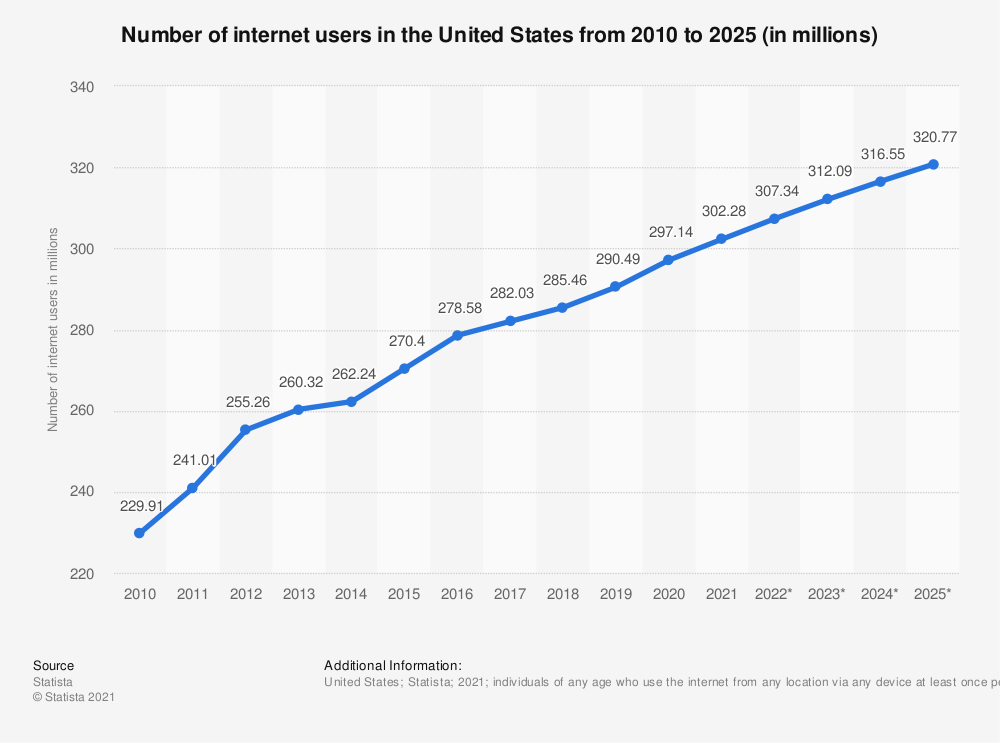
\includegraphics[width=0.8\textwidth]{number-of-internet-users}
\end{figure}
And not only have the number of internet users risen over the past eleven years, the average connection speed increased as well
over the same time period:
\begin{figure}[H]
    \centering
    \label{fig:internet-speed}
    \caption{Average internet connection speed in the US 2007-2017. \parencite{akamai2017}}
    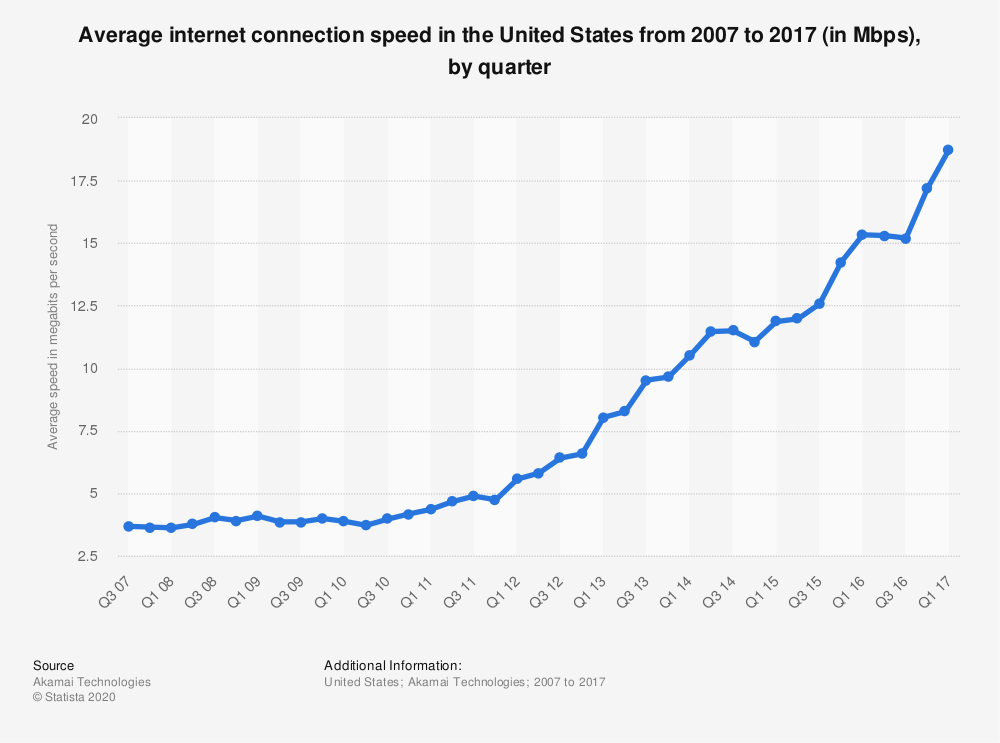
\includegraphics[width=0.8\textwidth]{internet-connection-speed}
\end{figure}
As seen above, from Q3 2017 to Q1 2017, average internet speeds across the US rose by 410\%.
This allowed for much more elaborate websites where larger amounts of data have to be downloaded.
Moreover, the number of robust frameworks for web development (be it front-end or back-end), make creating a complex web application easier
than ever before.
However, while this explains why SaaS is often the billing model of choice, it doesn't fully explain why specifically web applications
have risen in popularity. \parencite{statista2021}\par
After all, SaaS can also be delivered as a Desktop Application, as seen with the Adobe Creative Suite for example. \parencite{adobe2021}\par
To answer this, one should examine how desktop applications and web applications differ in more detail.

